%
% File main.tex
%
% Contact: car@ir.hit.edu.cn, gdzhou@suda.edu.cn
%%e.agirre@ehu.es or Sergi.Balari@uab.es
%% and that of ACL 08 by Joakim Nivre and Noah Smith

\documentclass[11pt]{article}
\usepackage{acl2015}
\usepackage{times}
\usepackage{latexsym}
\usepackage{graphicx}
\usepackage{listings}




\makeatletter
\newcommand{\@BIBLABEL}{\@emptybiblabel}
\newcommand{\@emptybiblabel}[1]{}
\makeatother
\usepackage[hyphens]{url}
\usepackage{hyperref}

%\setlength\titlebox{5cm}

% You can expand the title box if you need extra space
% to show all the authors. Please do not make the title box
% smaller than 5cm (the original size); we will check this
% in the camera-ready version and ask you to change it back.


\title{Spoiler detection and extraction pt. 2\\POC for NLP Course, Winter 2022/2023}

\author{M. Kierznowski, Ł. Pancer, P. Wesołowski \\
  Warsaw University of Technology \\
%   {\tt email@domain} \\
  \And
    supervisor: Anna Wróblewska \\
  Warsaw University of Technology \\
    {\tt anna.wroblewska1@pw.edu.pl}
    }

\date{}

\begin{document}
\maketitle
\begin{abstract}
This document presents exploratory data analysis, describes current experiments, and provides preliminary results for the second NLP course project. The project addresses the spoiler detection task. The main goal is to develop and evaluate architectures that are able to detect spoiler phrases within sentences. So far, we have focused on creating deep learning models based on LSTM networks.
\end{abstract}

\section{Introduction}

As an introduction, let us remind that in the previous project, we classified entire reviews as either containing spoilers or not. Then, we employed explainability tools to find the phrases that determined the classification of the entire review as a spoiler. In this project, we extend the previous work. Instead of teaching the models to classify entire reviews, we want to train them to extract spoiler phrases at the word level. Such a task may be viewed as a classification task since we aim to analyze models which classify every single word from a given input either as a spoiler or non-spoiler.

Since the problem posed in this way requires an accurately annotated dataset, we only have the option of using one of the three used in the previous project. We transform this dataset appropriately to fit our task. Finally, we perform some preliminary experiments with the LSTM-based deep learning model.

% We have shrunken our dataset number from three (from the previous project) to one, considering only  TV Tropes Books \cite{wroblewska2021spoiler}. This decision is dictated due to the fact that only this dataset fulfills our requirements. Primarily due to the word-based annotations.

Section \ref{literature} contains brief literature and currently employed LSTM model review. Section \ref{dataset} contains exploratory data analysis and transformation of the dataset. Finally, our preliminary experiment is described in section \ref{preliminary-model}.


\section{Literature}
\label{literature}

\subsection{Phrase extraction}
Our project idea was inspired by a medium article \cite{medium_extract}, an overview of a solution to a Twitter sentiment extraction Kaggle competition\cite{kaggle_comp}. The competition brought up the subject of extracting the exact part of a sentence responsible for its sentiment. For example, in a tweet, "my boss is bullying me," the phrase "bullying me" is directly responsible for its negative sentiment, as the rest of the sentence is neutral and could be used in a sentence of any sentiment. Unfortunately, this exact problem is, to our knowledge, non-existent in current literature. However, a lot can be discovered from problems of similar nature. 

Zhang \shortcite{zhang2011extracting} proposed a method for selecting words that do not bear sentiment on their own but only given context. For example, words describing resources may be positive or negative, e.g., "The washer uses a lot of electricity" or "The washer uses little water." In \cite{madasu2020efficient}, authors study the impact of a number of machine learning classifiers on the Term Frequency Inverse Document Frequency (TF-IDF) technique. Using feature selection combined techniques, they were able to outperform neural networks in sentiment analysis. Jianqiang et al. in \shortcite{jianqiang2018deep} applied a word embeddings method to sentiment analysis of Twitter posts. It's an improvement over TF-IDF because it extracts features such as contextual semantic relationships and co-occurrence statistical characteristics between words. Their approach, based on deep convolutional neural networks, outperformed the baseline word n-gram models. Yet another work \cite{rezaeinia2017improving} introduces an Improved Word Vectors (IWV) method, improving the accuracy of pretrained word embeddings. 


\subsection{Long short-term memory}
Long short-term memory (LSTM) architecture is an altered version of the recurrent neural networks (RNNs) that is able to learn long-term dependencies, mostly in sequence prediction problems. This type of network is used in speech recognition, machine translation, forecasting, etc.

Originally LSTM architecture was introduced in the work of Hochreiter, and Schmidhuber \shortcite{hochreiter1997long}. The main goal of LSTM is to mitigate the long-term dependency problem in comparison to the RNNs. 

The main structure of the LSTM network is depicted in figure \ref{fig:LSTModule}

\begin{figure}[h]
    \centering
    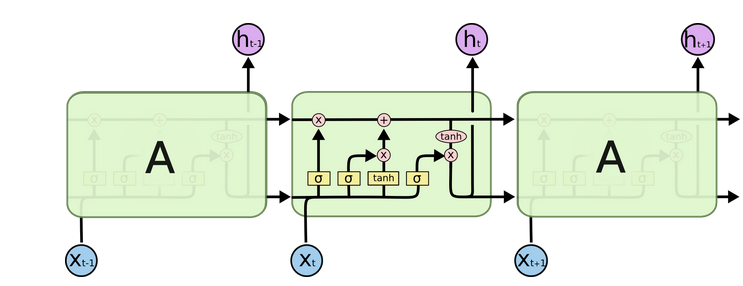
\includegraphics[width=\columnwidth]{img/LSTM.png}
    \caption{An example of LSTM module} 
    \label{fig:LSTModule}
\end{figure}

All LSTM networks have the form of a chain of repetitive modules. Contrary to an ordinary RNN block, LSTM consists of three different gates: a forget gate, an input gate, and an output gate. Those gates are crucial for obtaining long short-term memory in LSTM architecture. 


The first major challenge the LSTM tackles is what information consider redundant. For that issue, the forget gate comes to play. Example of forget gate is illustrated in figure \ref{fig:forgetGate}

\begin{figure}[h]
    \centering
    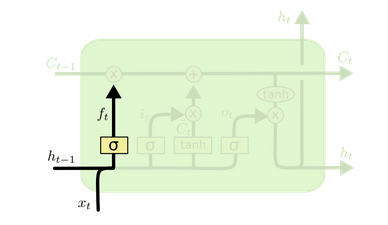
\includegraphics[width=\columnwidth]{img/ForgetGate.png}
    \caption{Forget gate} 
    \label{fig:forgetGate}
\end{figure}

The disregard of information is done by the sigmoid layer. Whereas 1 represents "completely keep this," a 0 represents "completely get rid of this." Afterward, the redundant information from the input and previous hidden state is discarded. 

Subsequently, the LSTM block uses the input gate, presented in figure \ref{fig:inputGate}, to determine what new information is going to be stored in the cell state. This has two parts. First, a sigmoid layer decides which values are being updated. Next, a tanh layer creates a vector of new candidate values that could be added to the state. In the final step, the LSTM cell combines them to create an update to the state.

\begin{figure}[h]
    \centering
    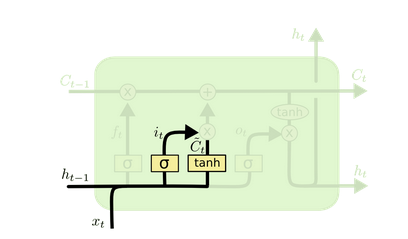
\includegraphics[width=\columnwidth]{img/InputGate.png}
    \caption{Input gate} 
    \label{fig:inputGate}
\end{figure}

Finally, LSTM uses a sigmoid layer that decides which parts of the input and hidden state will be considered as an output, which is shown in figure~\ref{fig:outputGate}. In addition, the tanh layer is utilized to map the cell state values into $[-1, 1]$ interval and multiply them by the output of the sigmoid.

\begin{figure}[h]
    \centering
    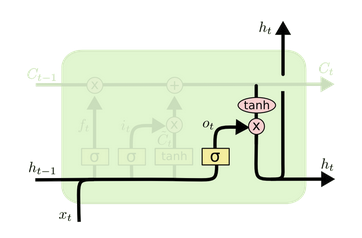
\includegraphics[width=\columnwidth]{img/outputGate.png}
    \caption{Output gate} 
    \label{fig:outputGate}
\end{figure}

Those improvements to the vanilla RNN's architectures resolve problems with long-term memory making the LSTM architectures superior in many tasks.

\section{Dataset} \label{dataset}
In our work, we needed a dataset that features word-level annotations. This need followed from the definition of the task. To our knowledge, only one dataset provides such annotations, namely the TV Tropes Books dataset\footnote{available at \url{https://github.com/rzepinskip/tvtropes-books}}. The dataset consists of precisely annotated reviews. In total, it contains 340k reviews with a 1:4 spoiler-to-non-spoiler review ratio. Among these, 670k sentences and 110k spoiler sentences are present. The dataset has already been split into the training, validation, and testing subsets. Note that in our architectures, we need text samples with a specified maximum number of words (tokens). That's why we modified this dataset to fit our needs. First, we present the exploratory data analysis, and then we describe obtaining the final dataset, adjusted to our task, that is used in the actual experiments.


\subsection{Exploratory data analysis} \label{eda}

The dataset contains serialized JSON objects. An example object corresponding to a single review is shown in the listing \ref{lst:sample-tvtropes-books}. Recall that our final model has a fixed input tokens count and the same size output vector. Therefore, our exploratory data analysis focuses on choosing the right strategy to transform this dataset into a form that meets our expectations. The following exploratory data analysis is based on the training part of the dataset.

\begin{minipage}{\linewidth}
\begin{lstlisting}[basicstyle=\small,caption={Sample truncated JSON object in the TV Tropes Books dataset. Each sentence contains a boolean flag that identifies spoiler sentences. In addition, annotated character indices provide specific spoiler boundaries.},label={lst:sample-tvtropes-books}]
{
'page': 'https://tvtropes.org/...',
'trope': 'Kill the Cutie',
'has_spoiler': True,
'sentences': [[True, 'Walter, who was
    the ...', [[0, 89]]]]
}
\end{lstlisting}
\end{minipage}

First, we decided to verify how many spoilers are annotated in a single sentence. Figure \ref{fig:spoilers-per-sentence} shows the corresponding histogram.

\begin{figure}
    \centering
    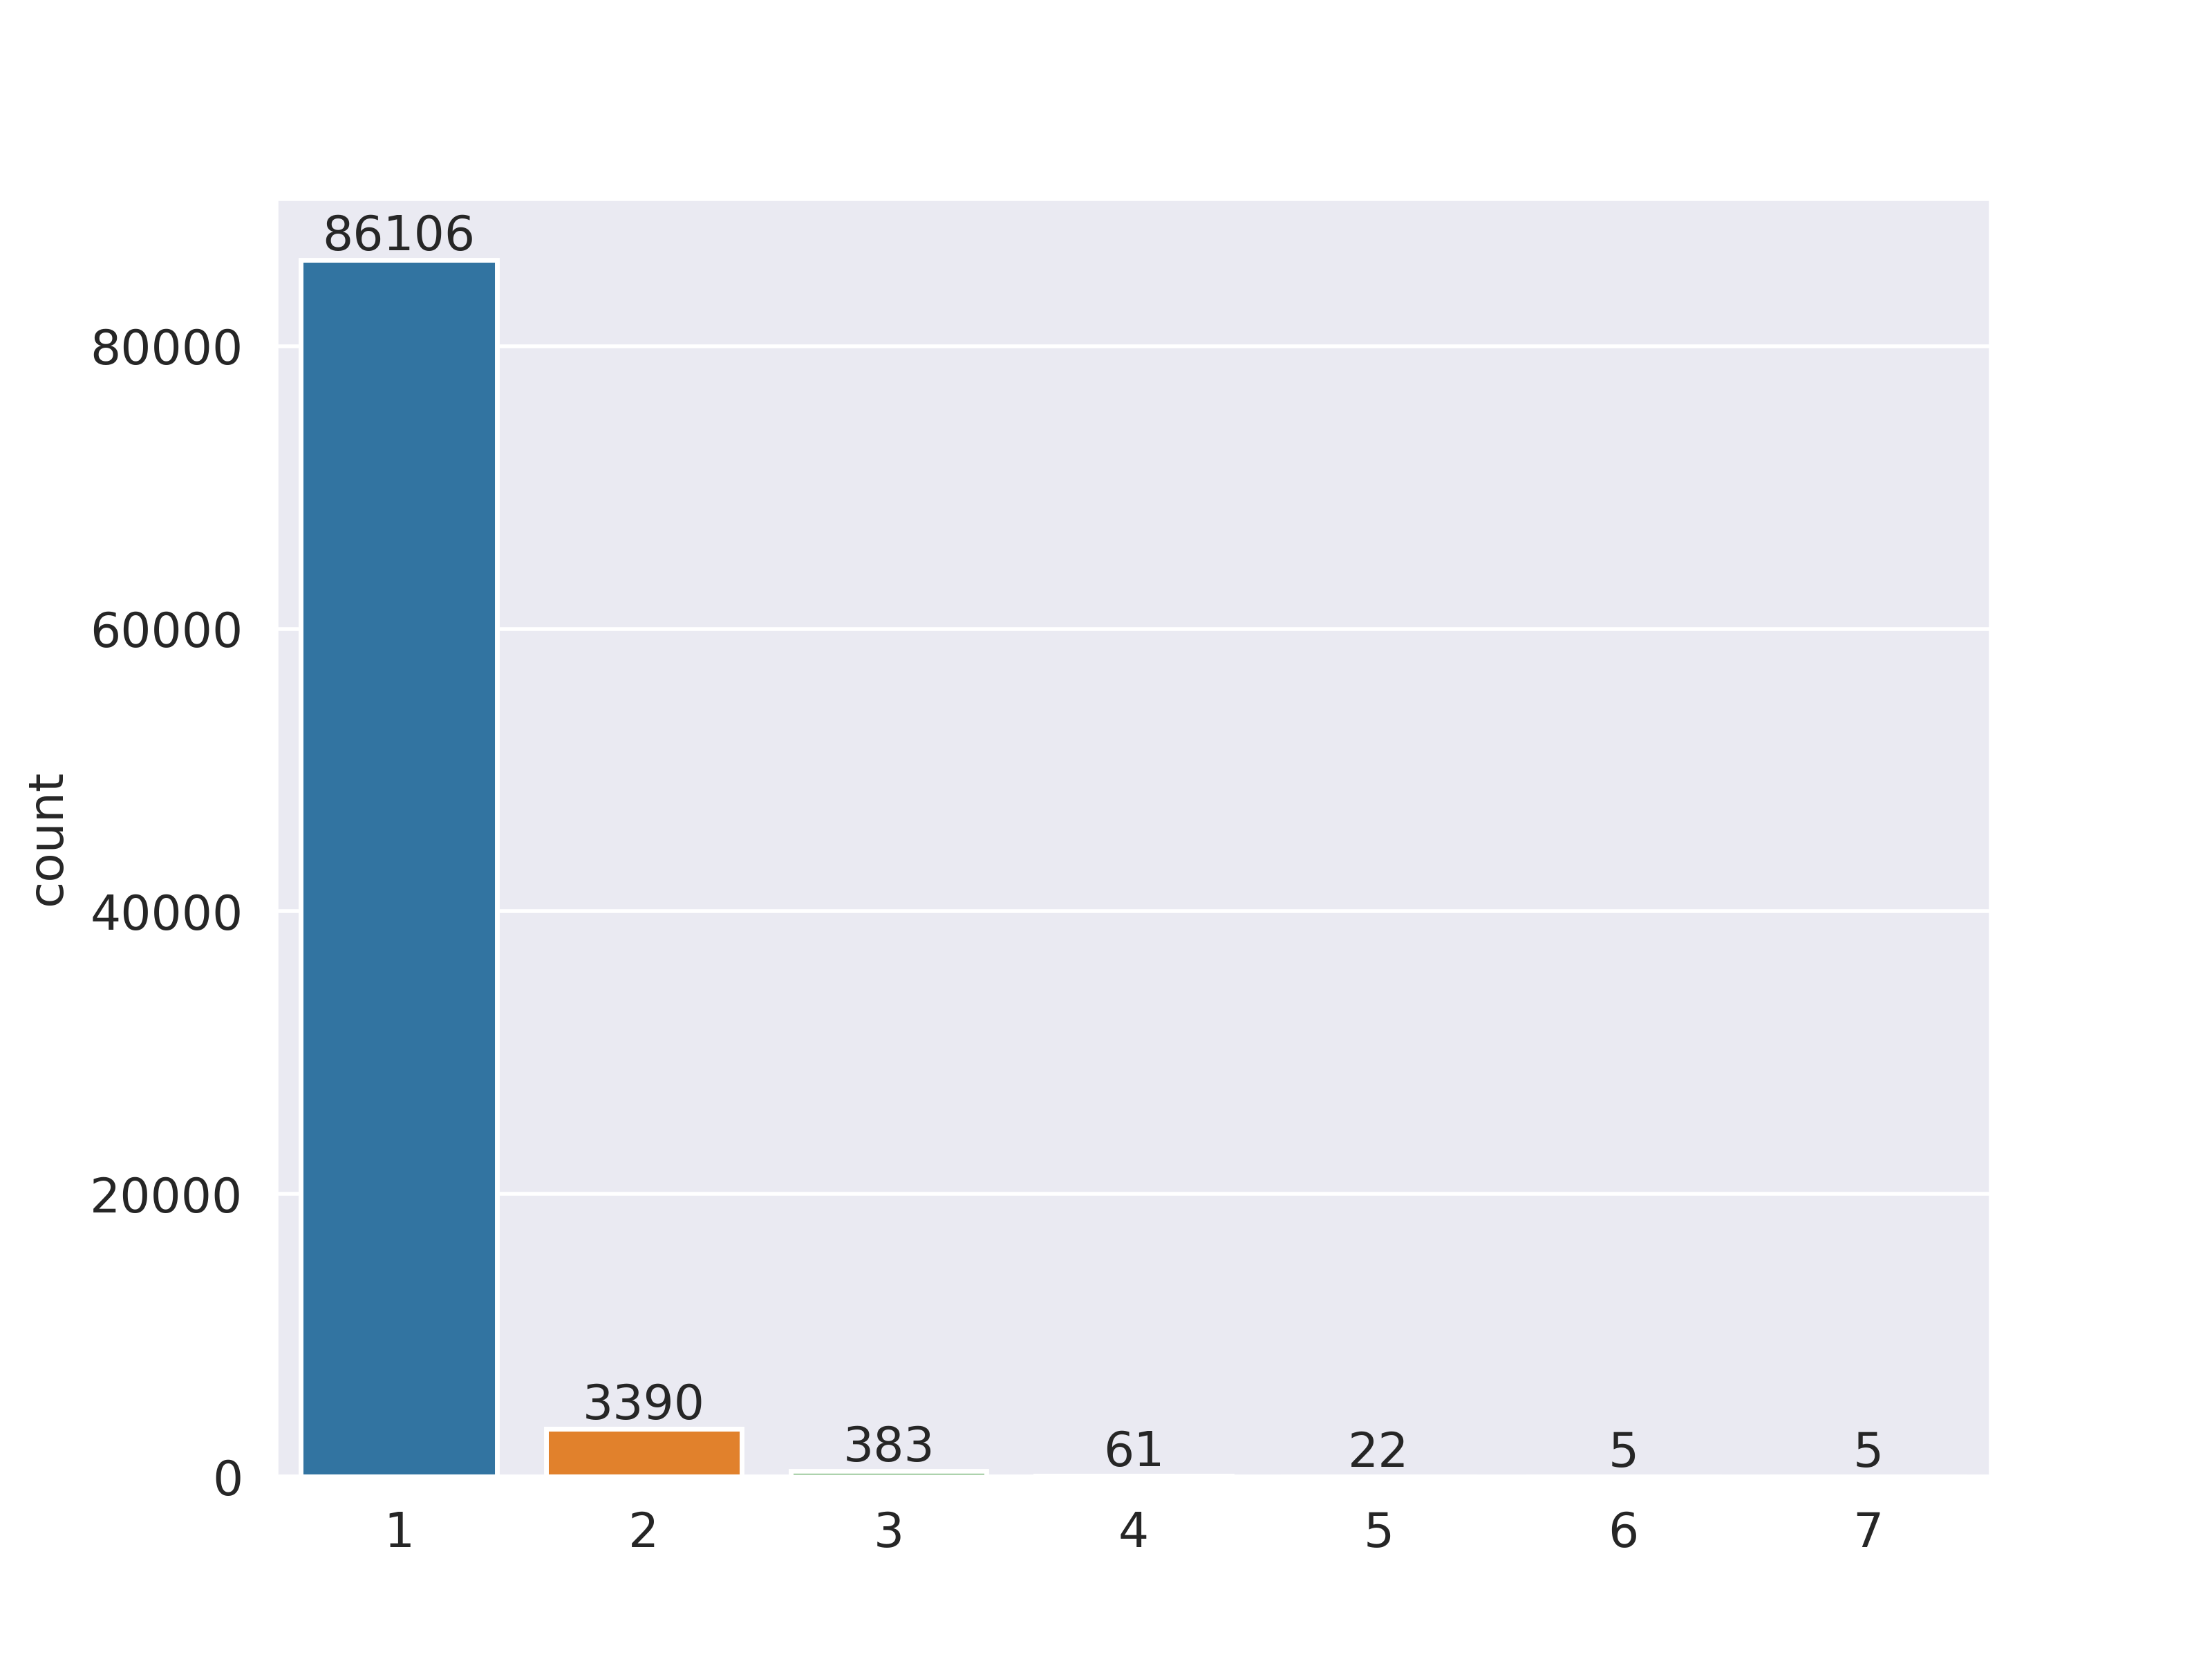
\includegraphics[width=\columnwidth]{img/eda/spoilers_per_sentence.png}
    \caption{Histogram presenting the distribution of spoiler counts within sentences. Note that only sentences with at least one spoiler are included. Sentences containing only one spoiler dominate.} 
    \label{fig:spoilers-per-sentence}
\end{figure}

Then, due to the expected fixed input word count, we focused on the histograms of the word count. Figure \ref{fig:words_count_per_spoiler_review} shows the histogram of word counts in the whole spoiler reviews. Another perspective is provided in figure \ref{fig:word_count_per_sentence_in_spoiler_review} depicting the histogram of word counts in sentences (only the sentences in spoiler reviews are considered). 

\begin{figure}
    \centering
    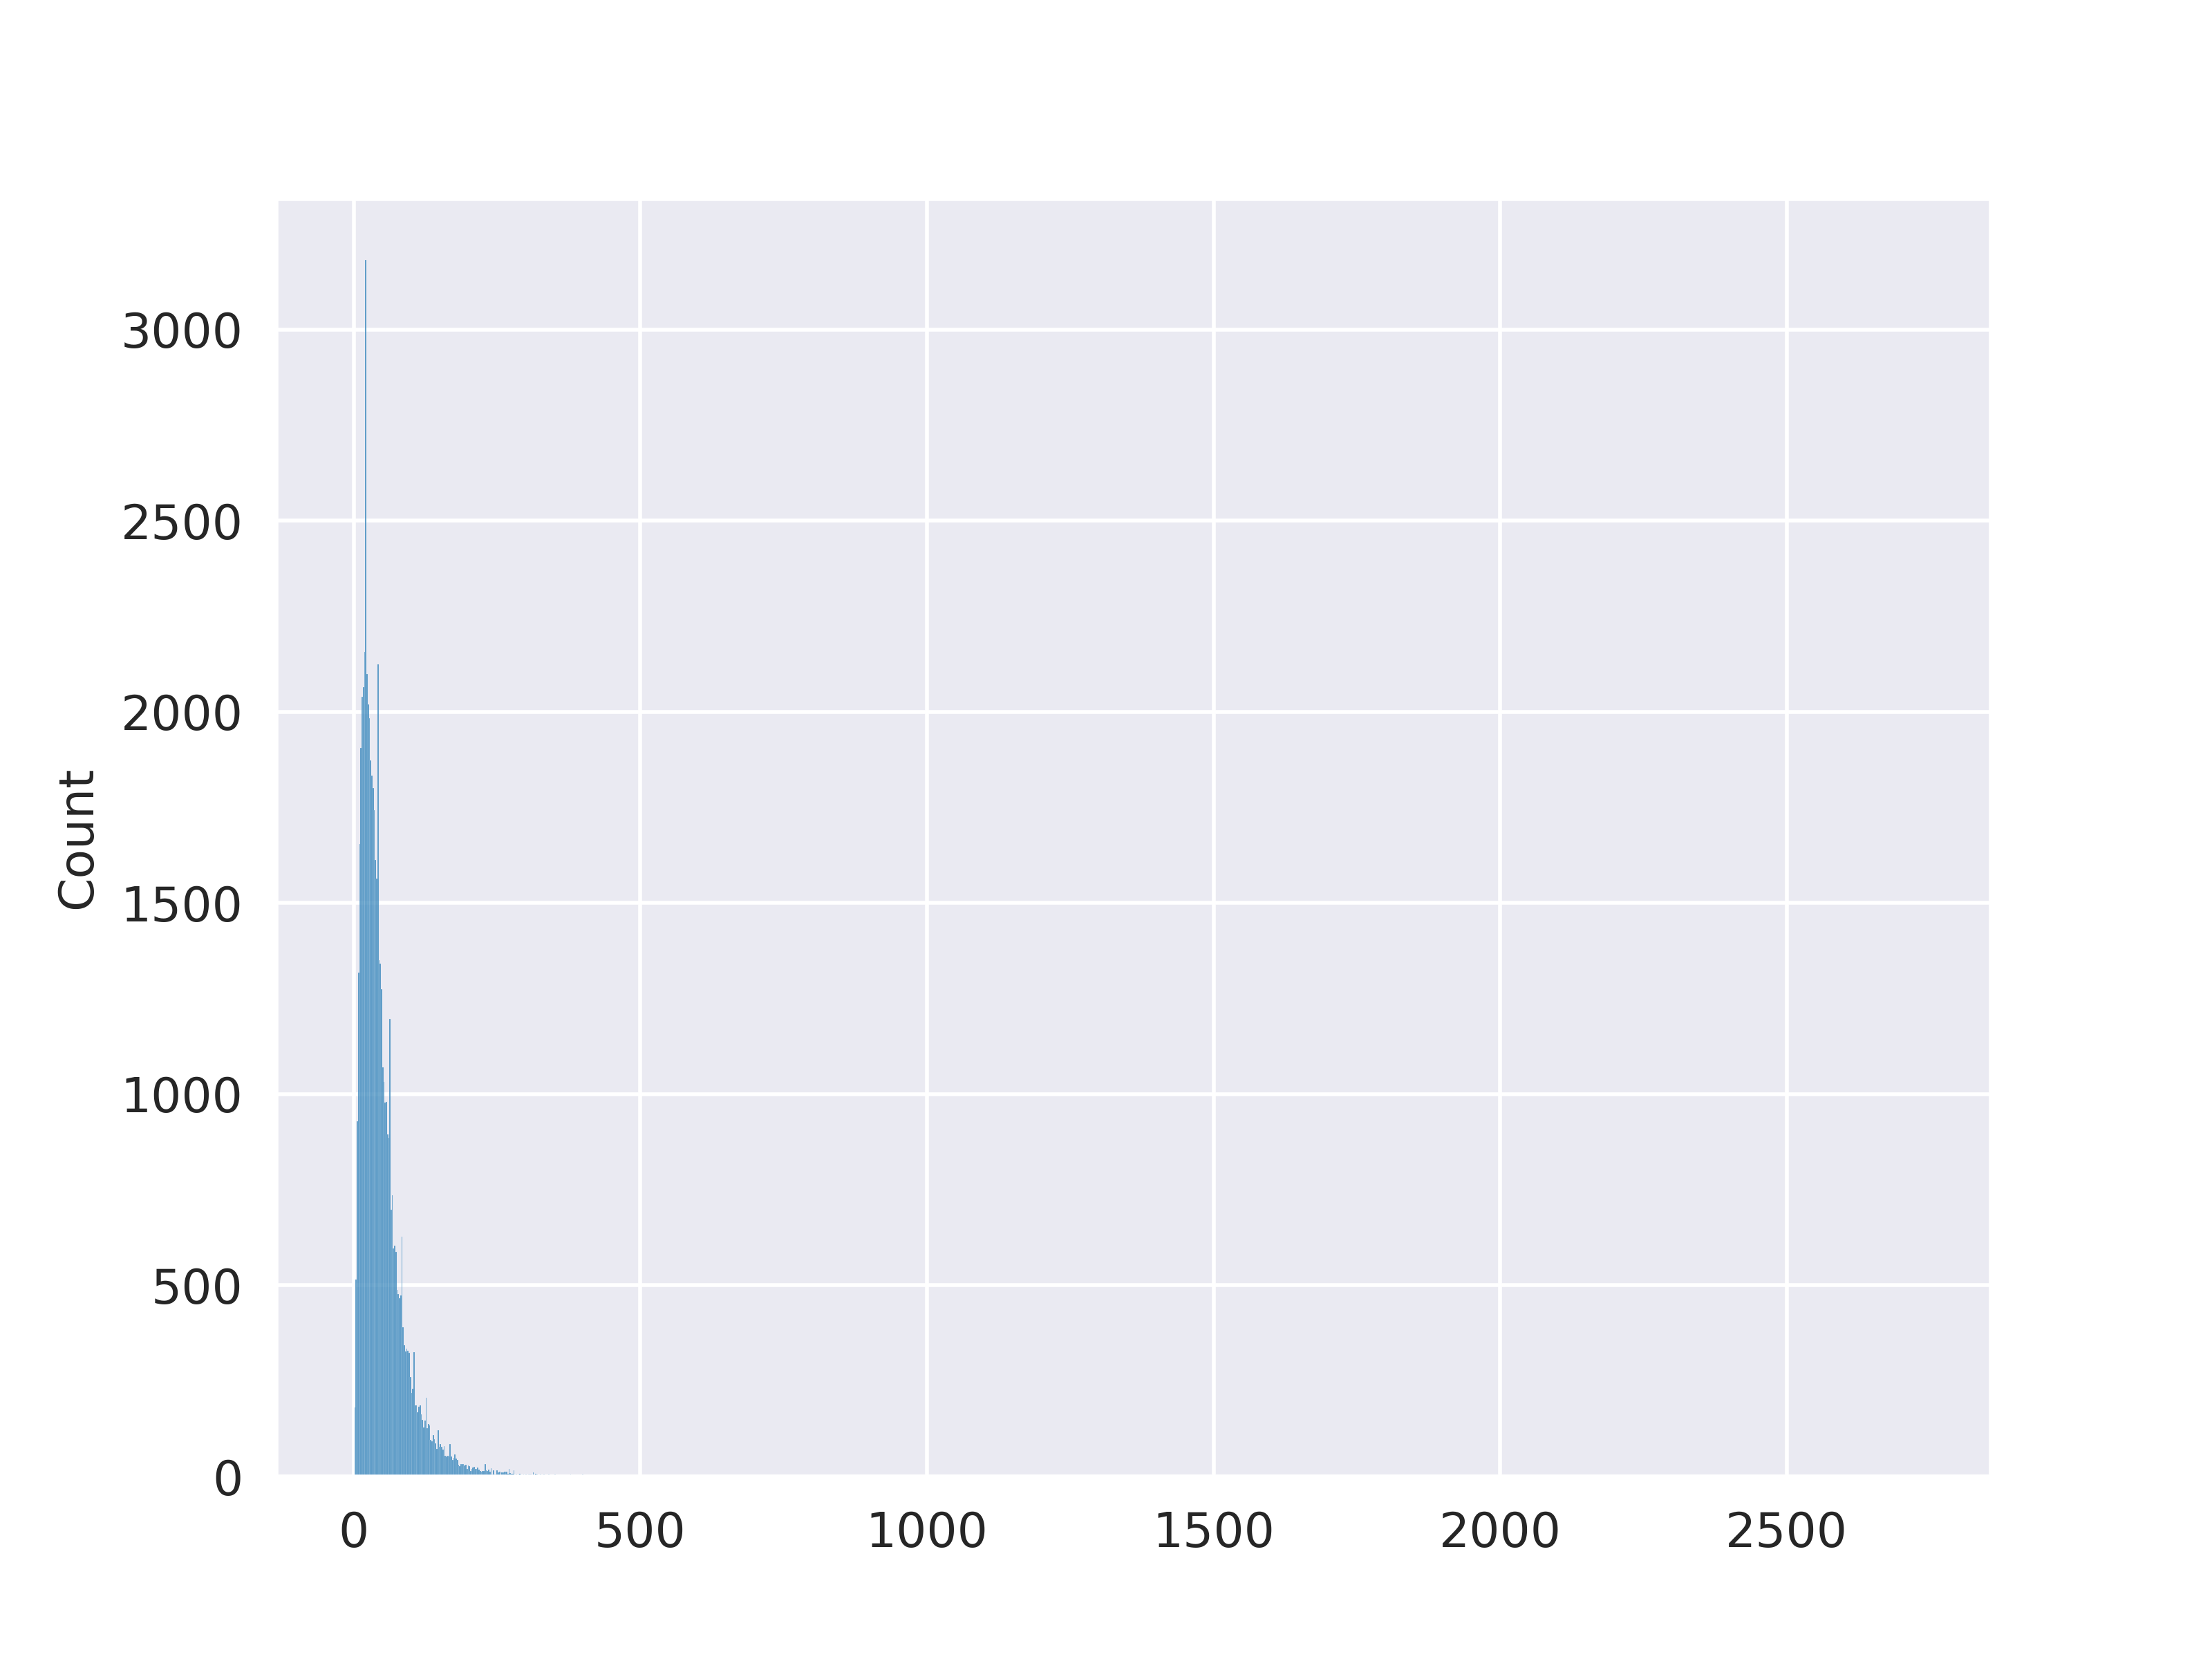
\includegraphics[width=\columnwidth]{img/eda/word_count_per_spoiler_review.png}
    \caption{Histogram presenting the distribution of word counts in whole spoiler reviews.} 
    \label{fig:words_count_per_spoiler_review}
\end{figure}

\begin{figure}
    \centering
    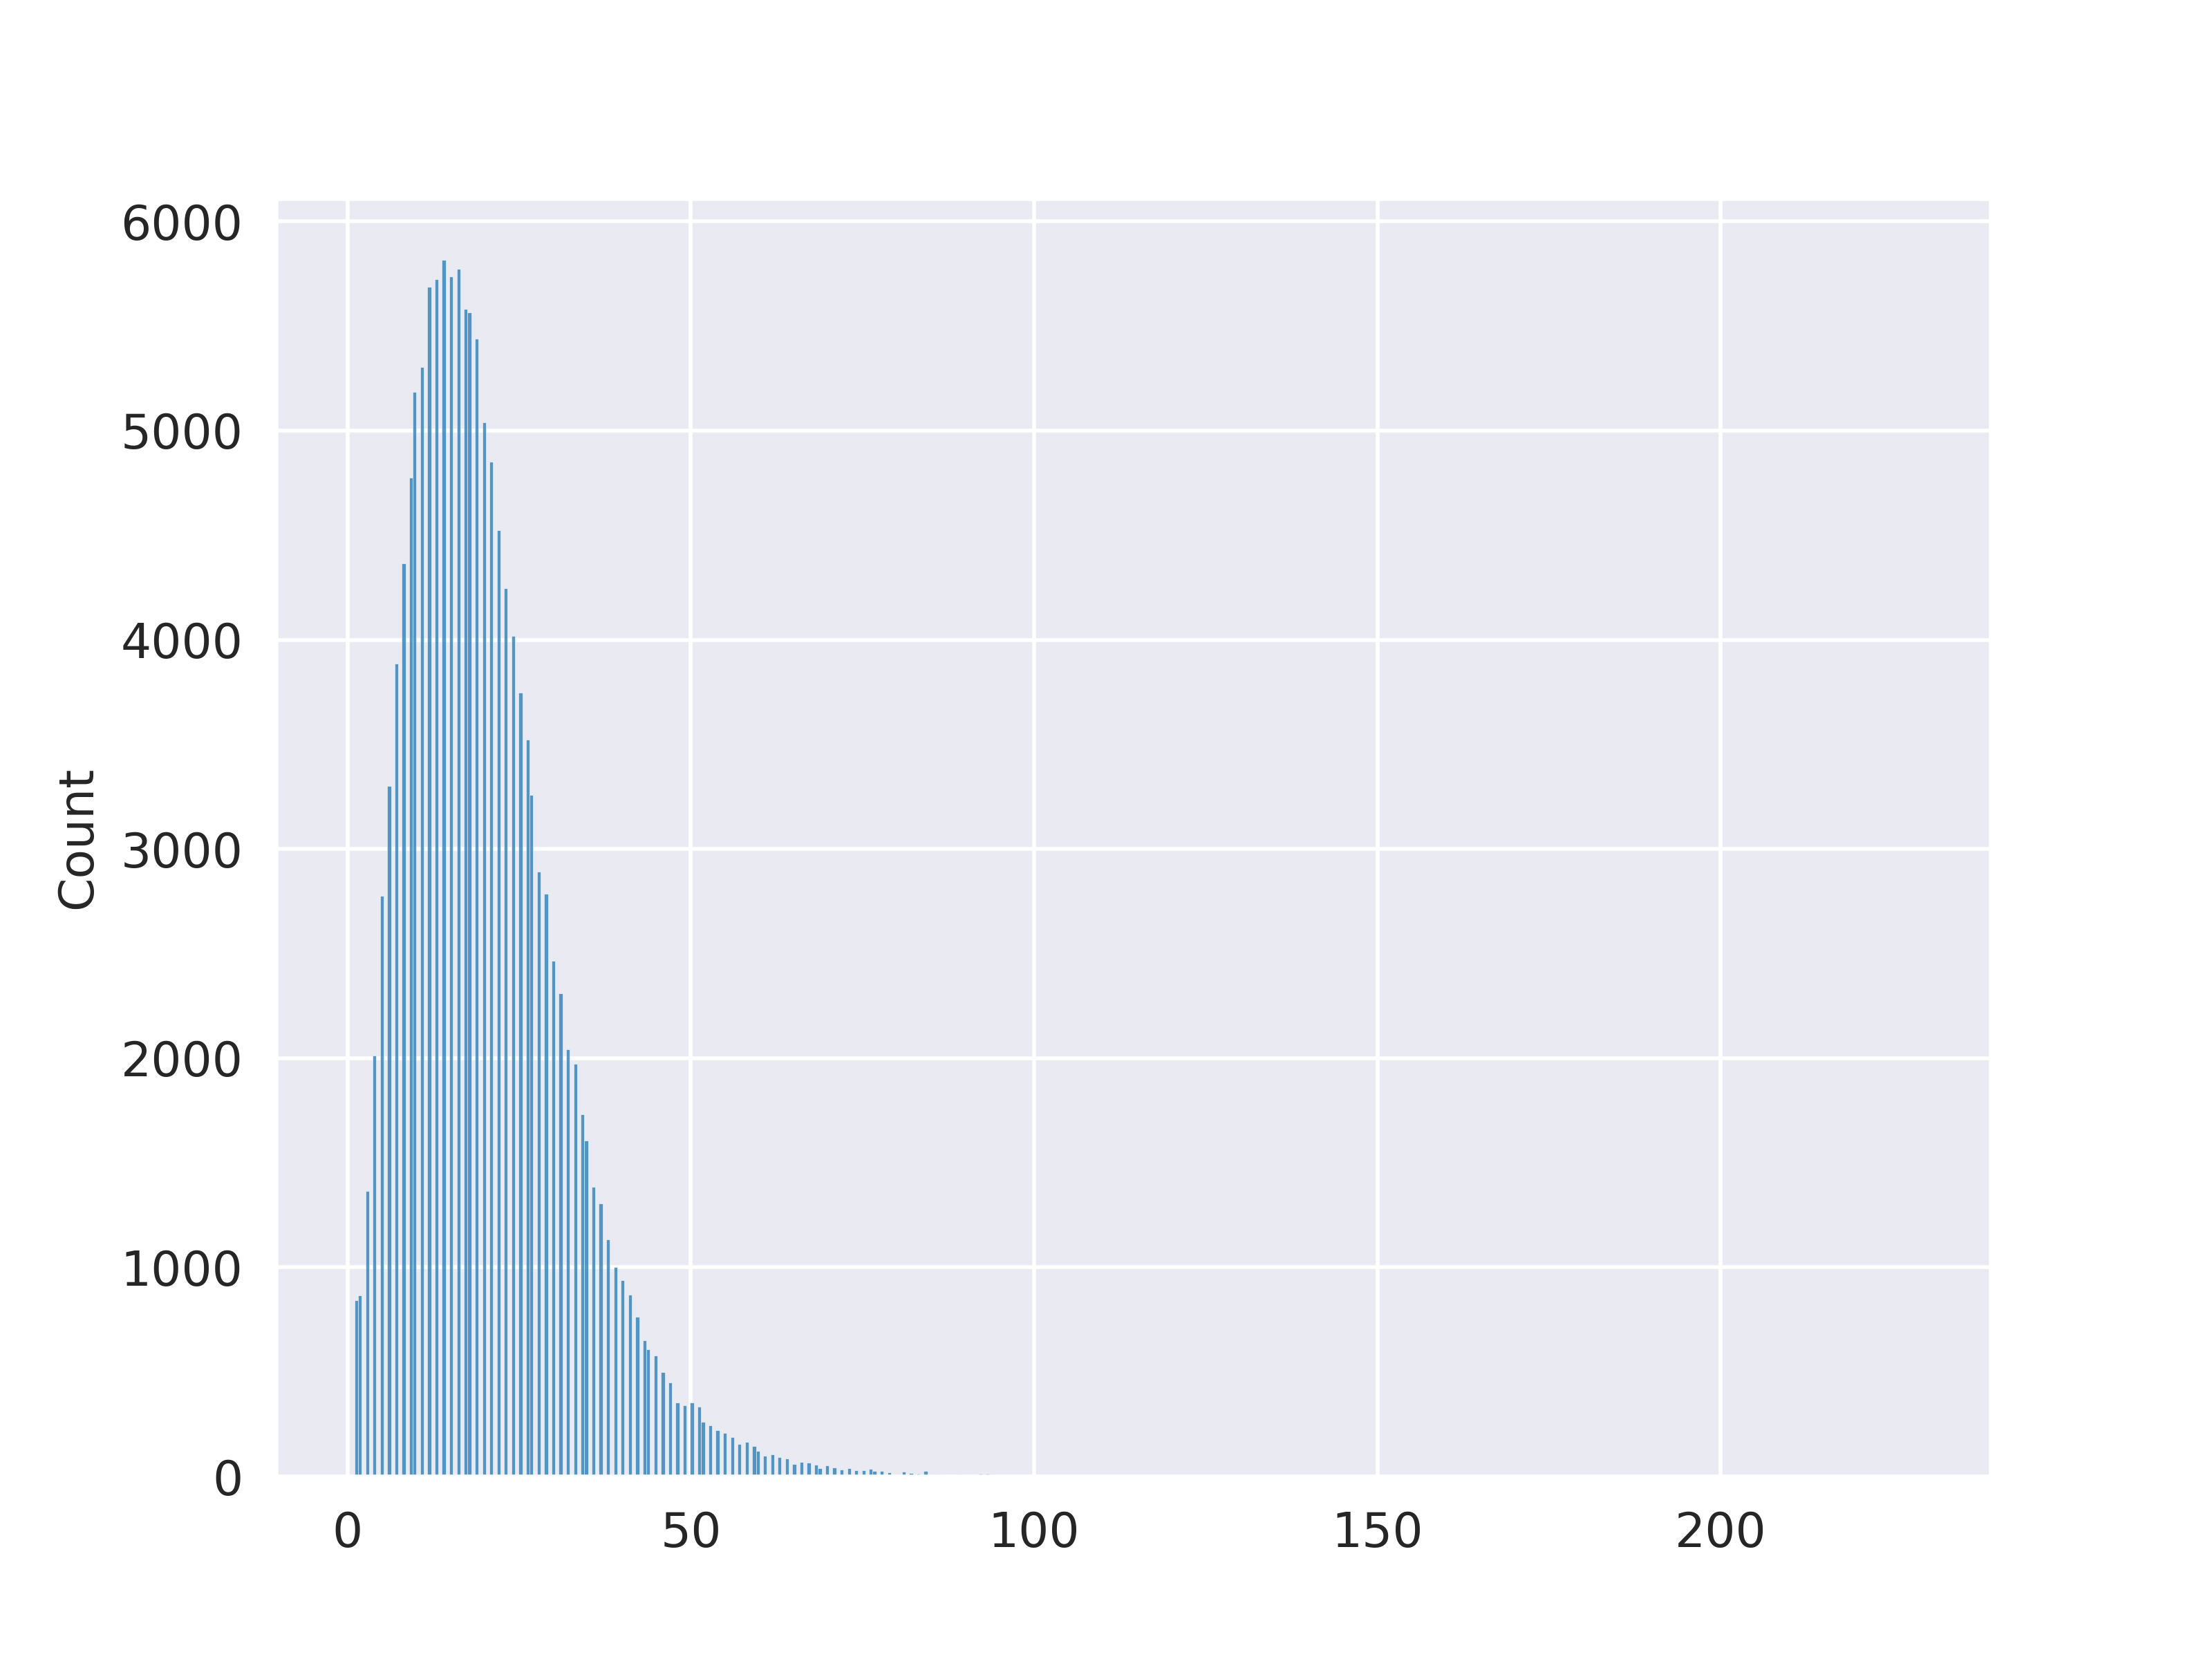
\includegraphics[width=\columnwidth]{img/eda/word_count_per_sencence_in_spoiler_review.png}
    \caption{Histogram presenting the distribution of word counts in sentences. The sentences come from spoiler reviews.} 
    \label{fig:word_count_per_sentence_in_spoiler_review}
\end{figure}

As we were looking for an idea of how to transform the collection appropriately to get review fragments with a certain maximum word count, we decided to check where in the sentences the spoilers end up. The result is shown in figure~\ref{fig:on_which_word_in_sentence_spoiler_ends}.
\begin{figure}
    \centering
    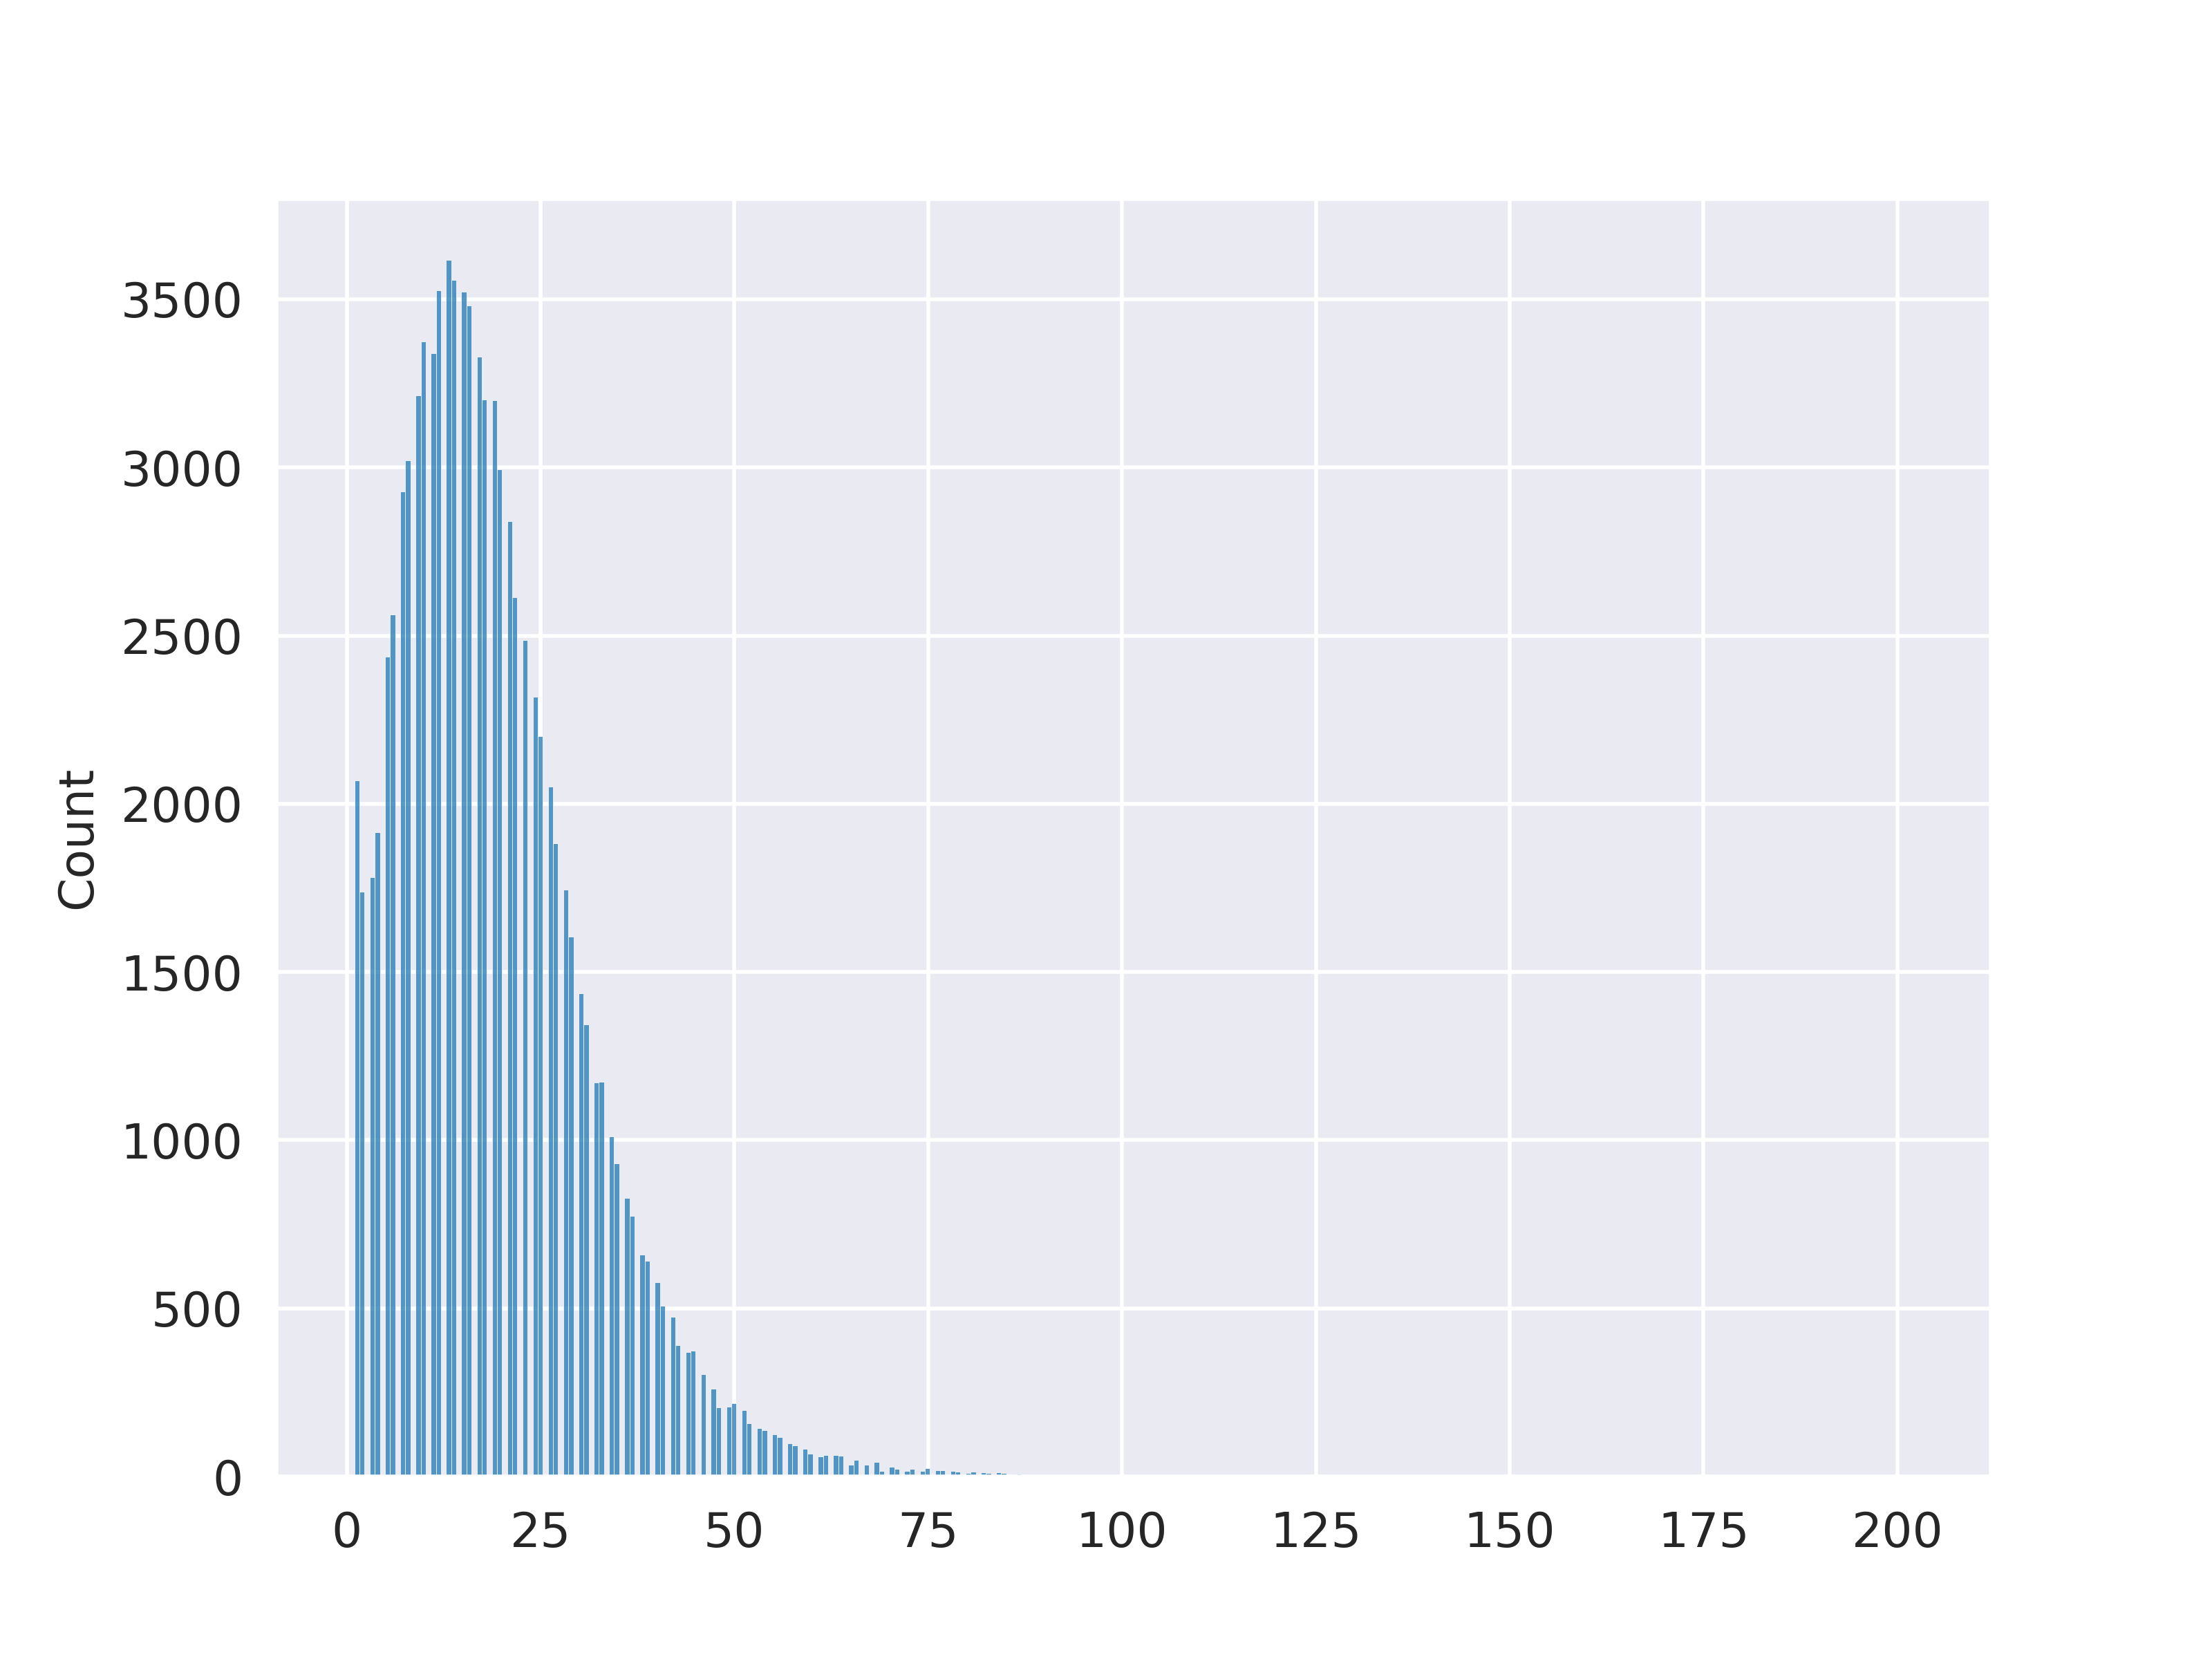
\includegraphics[width=\columnwidth]{img/eda/on_which_word_in_sentence_spoiler_ends.png}
    \caption{Histogram presenting the distribution of the last spoiler word inside a spoiler sentence.} 
    \label{fig:on_which_word_in_sentence_spoiler_ends}
\end{figure}

The similarity of figures \ref{fig:word_count_per_sentence_in_spoiler_review} and \ref{fig:on_which_word_in_sentence_spoiler_ends} seemed suspicious to us. Therefore, we decided to verify what fractions of spoiler sentences are actually annotated as spoilers. For every spoiler sentence, the number of words annotated as spoilers is divided by the number of words in the sentence. The histogram shown in figure \ref{fig:how_much_of_spoiler_is_in_spoiler_sentence} shows the distribution of these fractions.

\begin{figure}
    \centering
    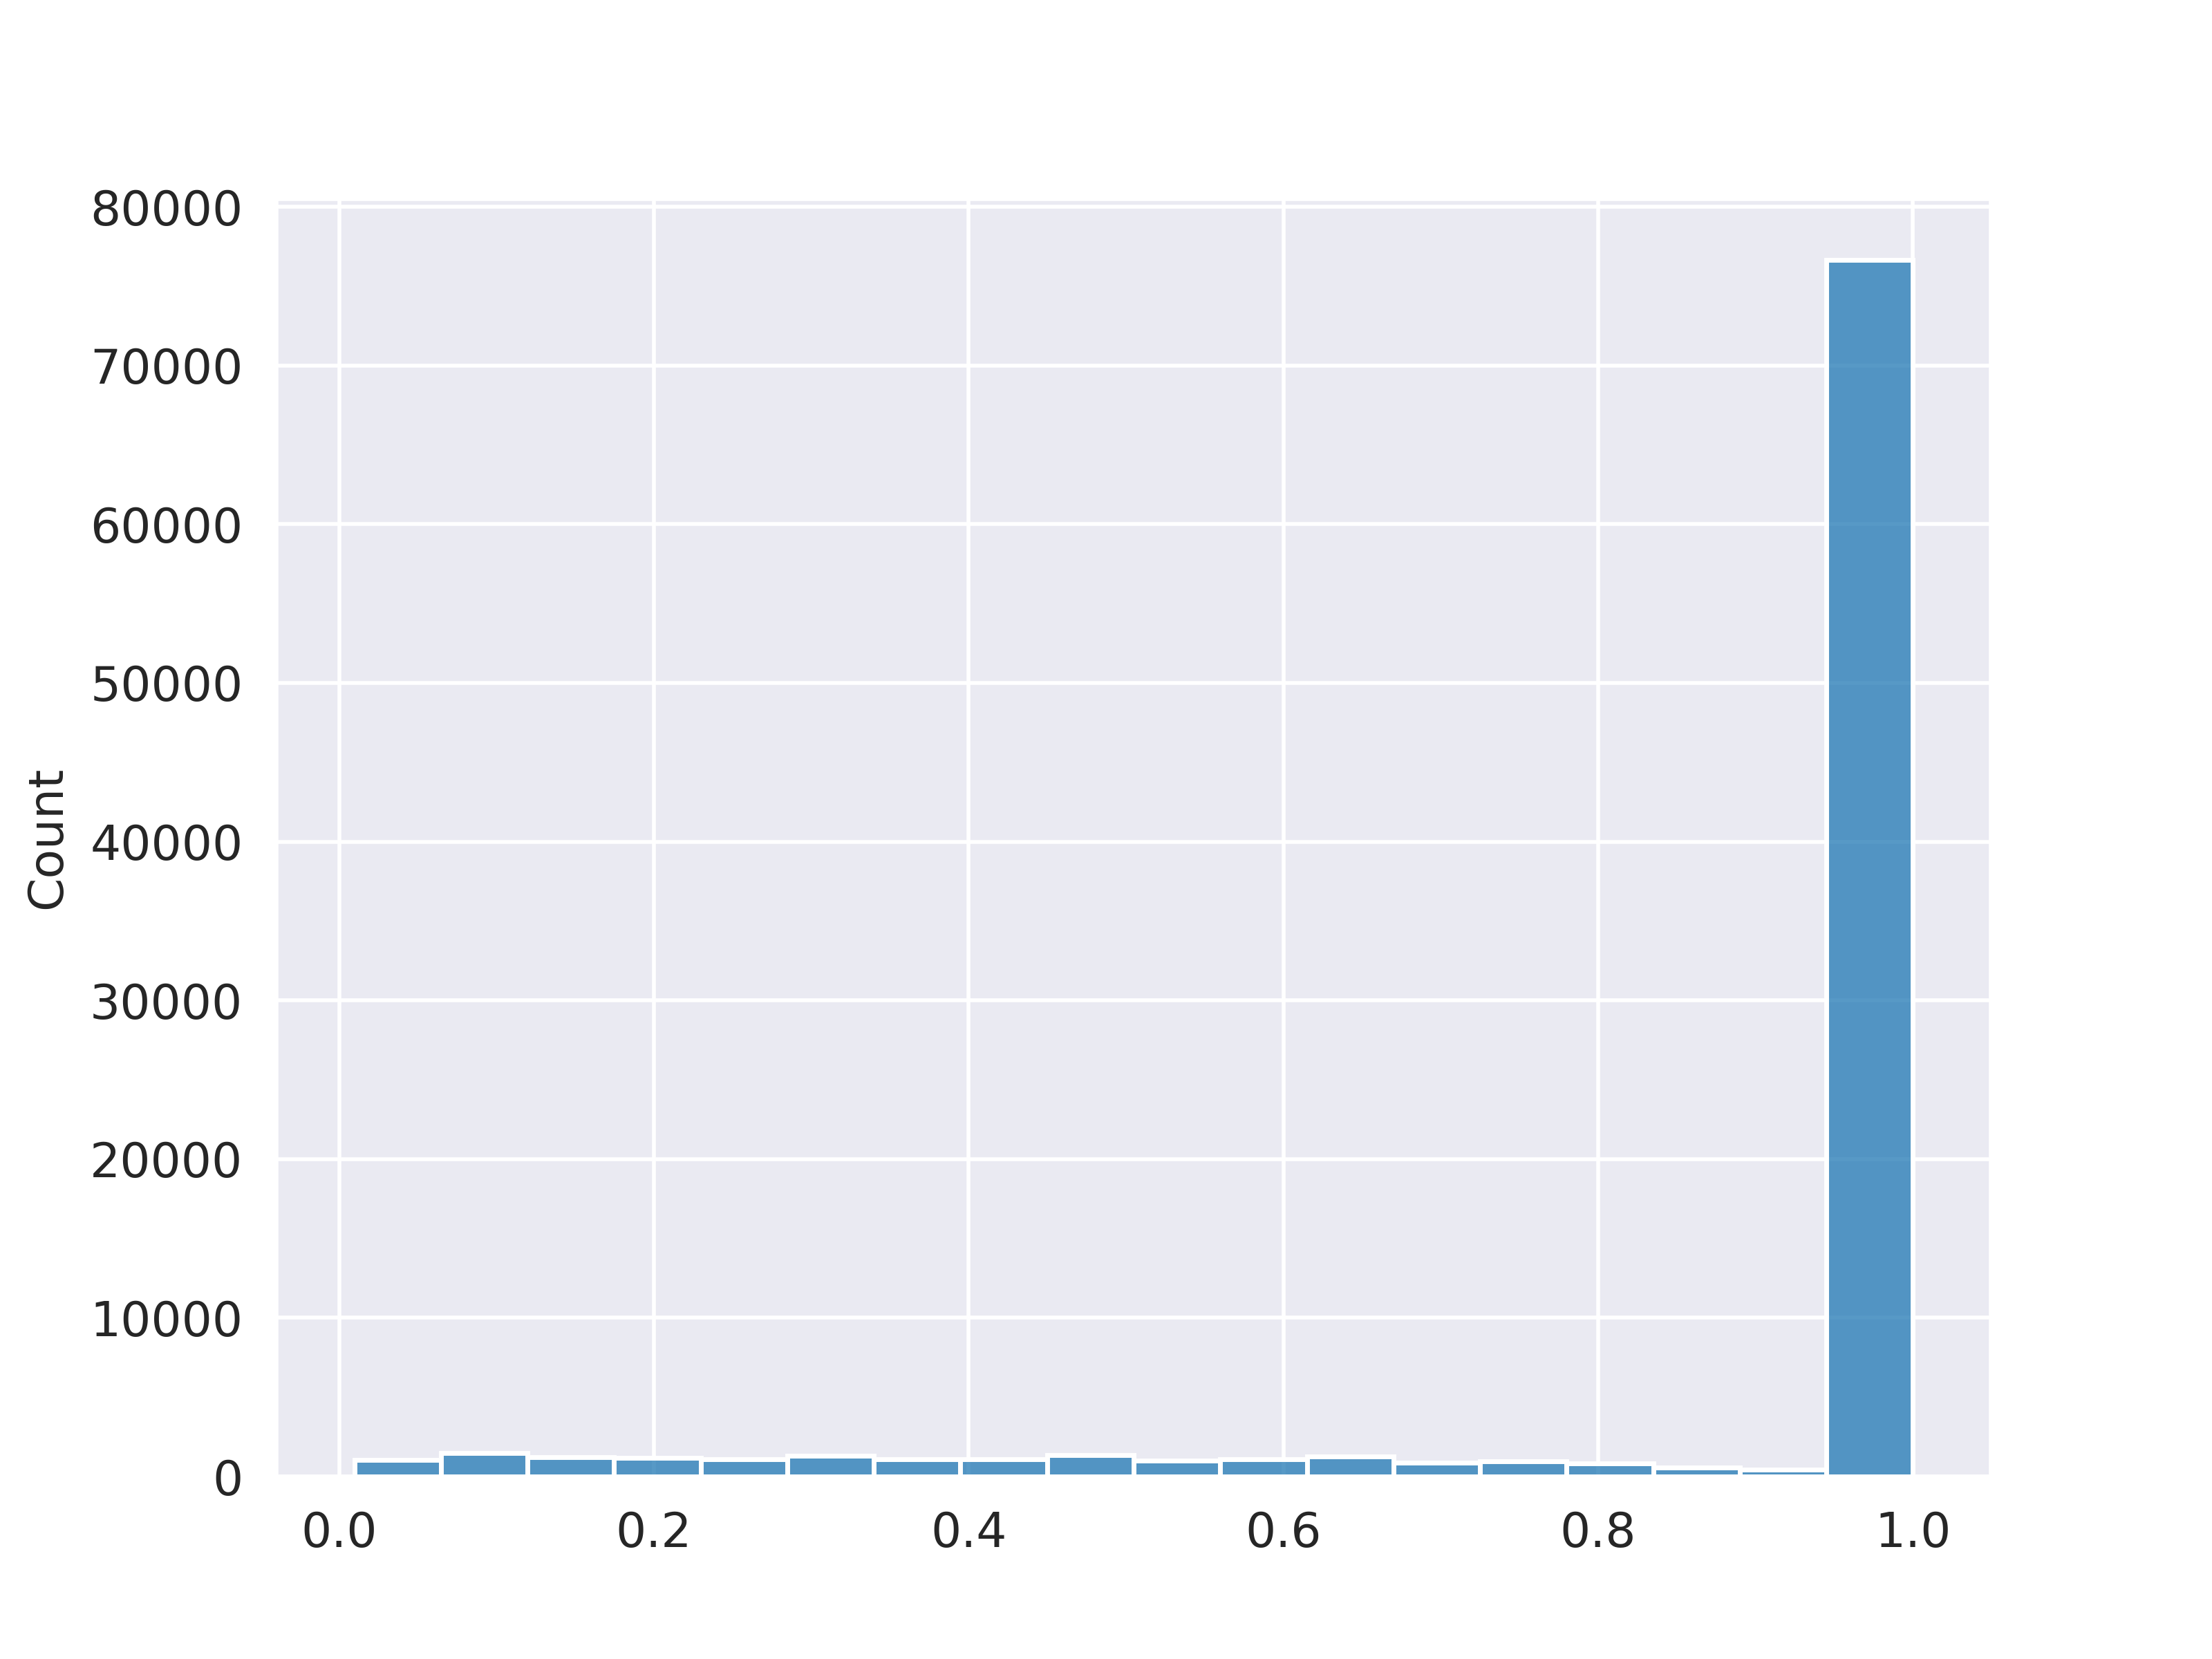
\includegraphics[width=\columnwidth]{img/eda/how_much_of_spoiler_is_in_spoiler_sentence.png}
    \caption{Histogram presenting the distribution of the fraction of spoiler words in spoiler sentences.} 
    \label{fig:how_much_of_spoiler_is_in_spoiler_sentence}
\end{figure}

The plot presented in figure \ref{fig:how_much_of_spoiler_is_in_spoiler_sentence} may be surprising. It turns out that in the vast majority, entire sentences are spoilers. We do not know whether this is due to fairly general tagging by portal users who have tagged whole sentences or whether whole sentences are actually spoilers.

\subsection{Dataset transformation}

The above exploratory data analysis led us to decide to finally transform the dataset in a straightforward manner. Recall that we had to make sure that our input samples were not longer than the specified number of tokens. The algorithm is as follows. For every spoiler review, perform the following operations:
\begin{enumerate}
\item Concatenate sentences as long as they are within the maximum number of words.
\item Add concatenated sentences to the final dataset.
\item If some sentences from the review considered have not been included in the result, go back to 1. and start concatenating them.
\end{enumerate}
Of course, single sentences that are longer on their own than the maximum number of words allowed are not included in the resulting dataset. It is worth noting that this transformation must be combined with procedures typically performed by a tokenizer, such as splitting. It's due to the need to track the positions of spoiler words. Therefore, simultaneously with the concatenation operations, the target label vector is created. The length of the vector equals the number of words in the corresponding review fragment. Such a vector contains boolean flags indicating spoiler words. Example data and corresponding target vector are presented in listing \ref{lst:sample-final-data}. 

\begin{figure*}[t]
\begin{lstlisting}[basicstyle=\small,caption={Sample element of the dataset adjusted to our needs. The maximum number of tokens was 64. Note that the text has already undergone preprocessing, e.g., punctuation removal. The target vector is a boolean vector indicating spoiler words. In this case, \textit{and can't bear him children} was annotated as a spoiler phrase.},label={lst:sample-final-data}]
("celia is this to johnny because he's from a rich well to do family while she's
white trash from sugar ditch and doesn't know how to cook clean and can't bear him
children",
 [False, False, ..., False, True, True, True, True, True])
\end{lstlisting}
\end{figure*}


\section{Preliminary architecture} \label{preliminary-model}

Since we were afraid of the computational complexity, we selected the maximum length of review fragments to be 64 tokens. We ended up with about 47k review fragments that contained both spoiler and non-spoiler phrases, 20k fragments containing only spoiler words, and 12k fragments with no spoilers. Therefore, our final training dataset features about 79k labeled review fragments. 

Before describing specific layers of the model, some key data transformation has to be prepared. For samples that contain less than 64 words, we applied zero padding such that every document length is the same, equal to 64. After those necessary prepossessing, architecture is able to consume the data.

The architecture consists of an LSTM layer which is preceded by an embeddings layer. This specific object transfers tokenized input to its embedded value. As weights, we utilize GloVe embeddings, and those weights are frozen (they are no longer trainable). Since our model aims to classify every word, it might be considered a sequence-to-sequence model. Therefore, the number of neurons in the last layer corresponds to the maximum number of input words (in provided case, 64). This first approach, combined with independently applied sigmoid function, gave us satisfactory results. On the testing set, we achieved $0.8169$ accuracy, where accuracy is considered per each word. Apart from that, we also implemented the Jaccard similarity score, which gave us a $0.7811$ set similarity for non-spoiler words and $0.4718$ set similarity for spoiler words. The exact hyperparameters, etc., will be provided in the final report because we may change the model, etc.


\section{Summary}
In this document, we have shown our current progress. The next step is to increase the input and output vector size (from 64 to, probably, 512 - recall figure \ref{fig:words_count_per_spoiler_review}). In addition, we will test different models.


% include your bib file like this:
\bibliographystyle{acl}
\bibliography{bibliography}

\end{document}